\documentclass[a4paper]{letter}
\usepackage{wallpaper}
\usepackage{geometry}
\usepackage{xcolor}
\usepackage[T1]{fontenc}
\usepackage[scaled]{helvet}
\usepackage{fontawesome5}
\usepackage[hidelinks]{hyperref}
\usepackage[english]{babel}
\usepackage{graphicx}
\usepackage{tikz}
\usepackage{setspace}
\usepackage{comment}

\usetikzlibrary{calc}

\renewcommand{\familydefault}{\sfdefault}

\geometry{
  a4paper,
  left=20pt,
  right=20pt,
  top=0pt,
  bottom=0pt,
  nohead,
  nofoot,
  nomarginpar
}

\ThisCenterWallPaper{1.1}{cvbg.png}

% Custom command for dividers
\newcommand{\divider}{\rule{\linewidth}{0.9pt}}

% ============================================================
% ======================== Left Side =========================
% ============================================================

\begin{document}

%\small
\begin{minipage}[t]{0.40\textwidth}
\setstretch{1.2} 
\setlength{\baselineskip}{1\baselineskip}
\color{white}
\vspace{4mm}

% ========================== Photo ============================

\begin{tikzpicture}
    \clip (0,0) circle (2cm);
    \node[anchor=center] at (0,0) {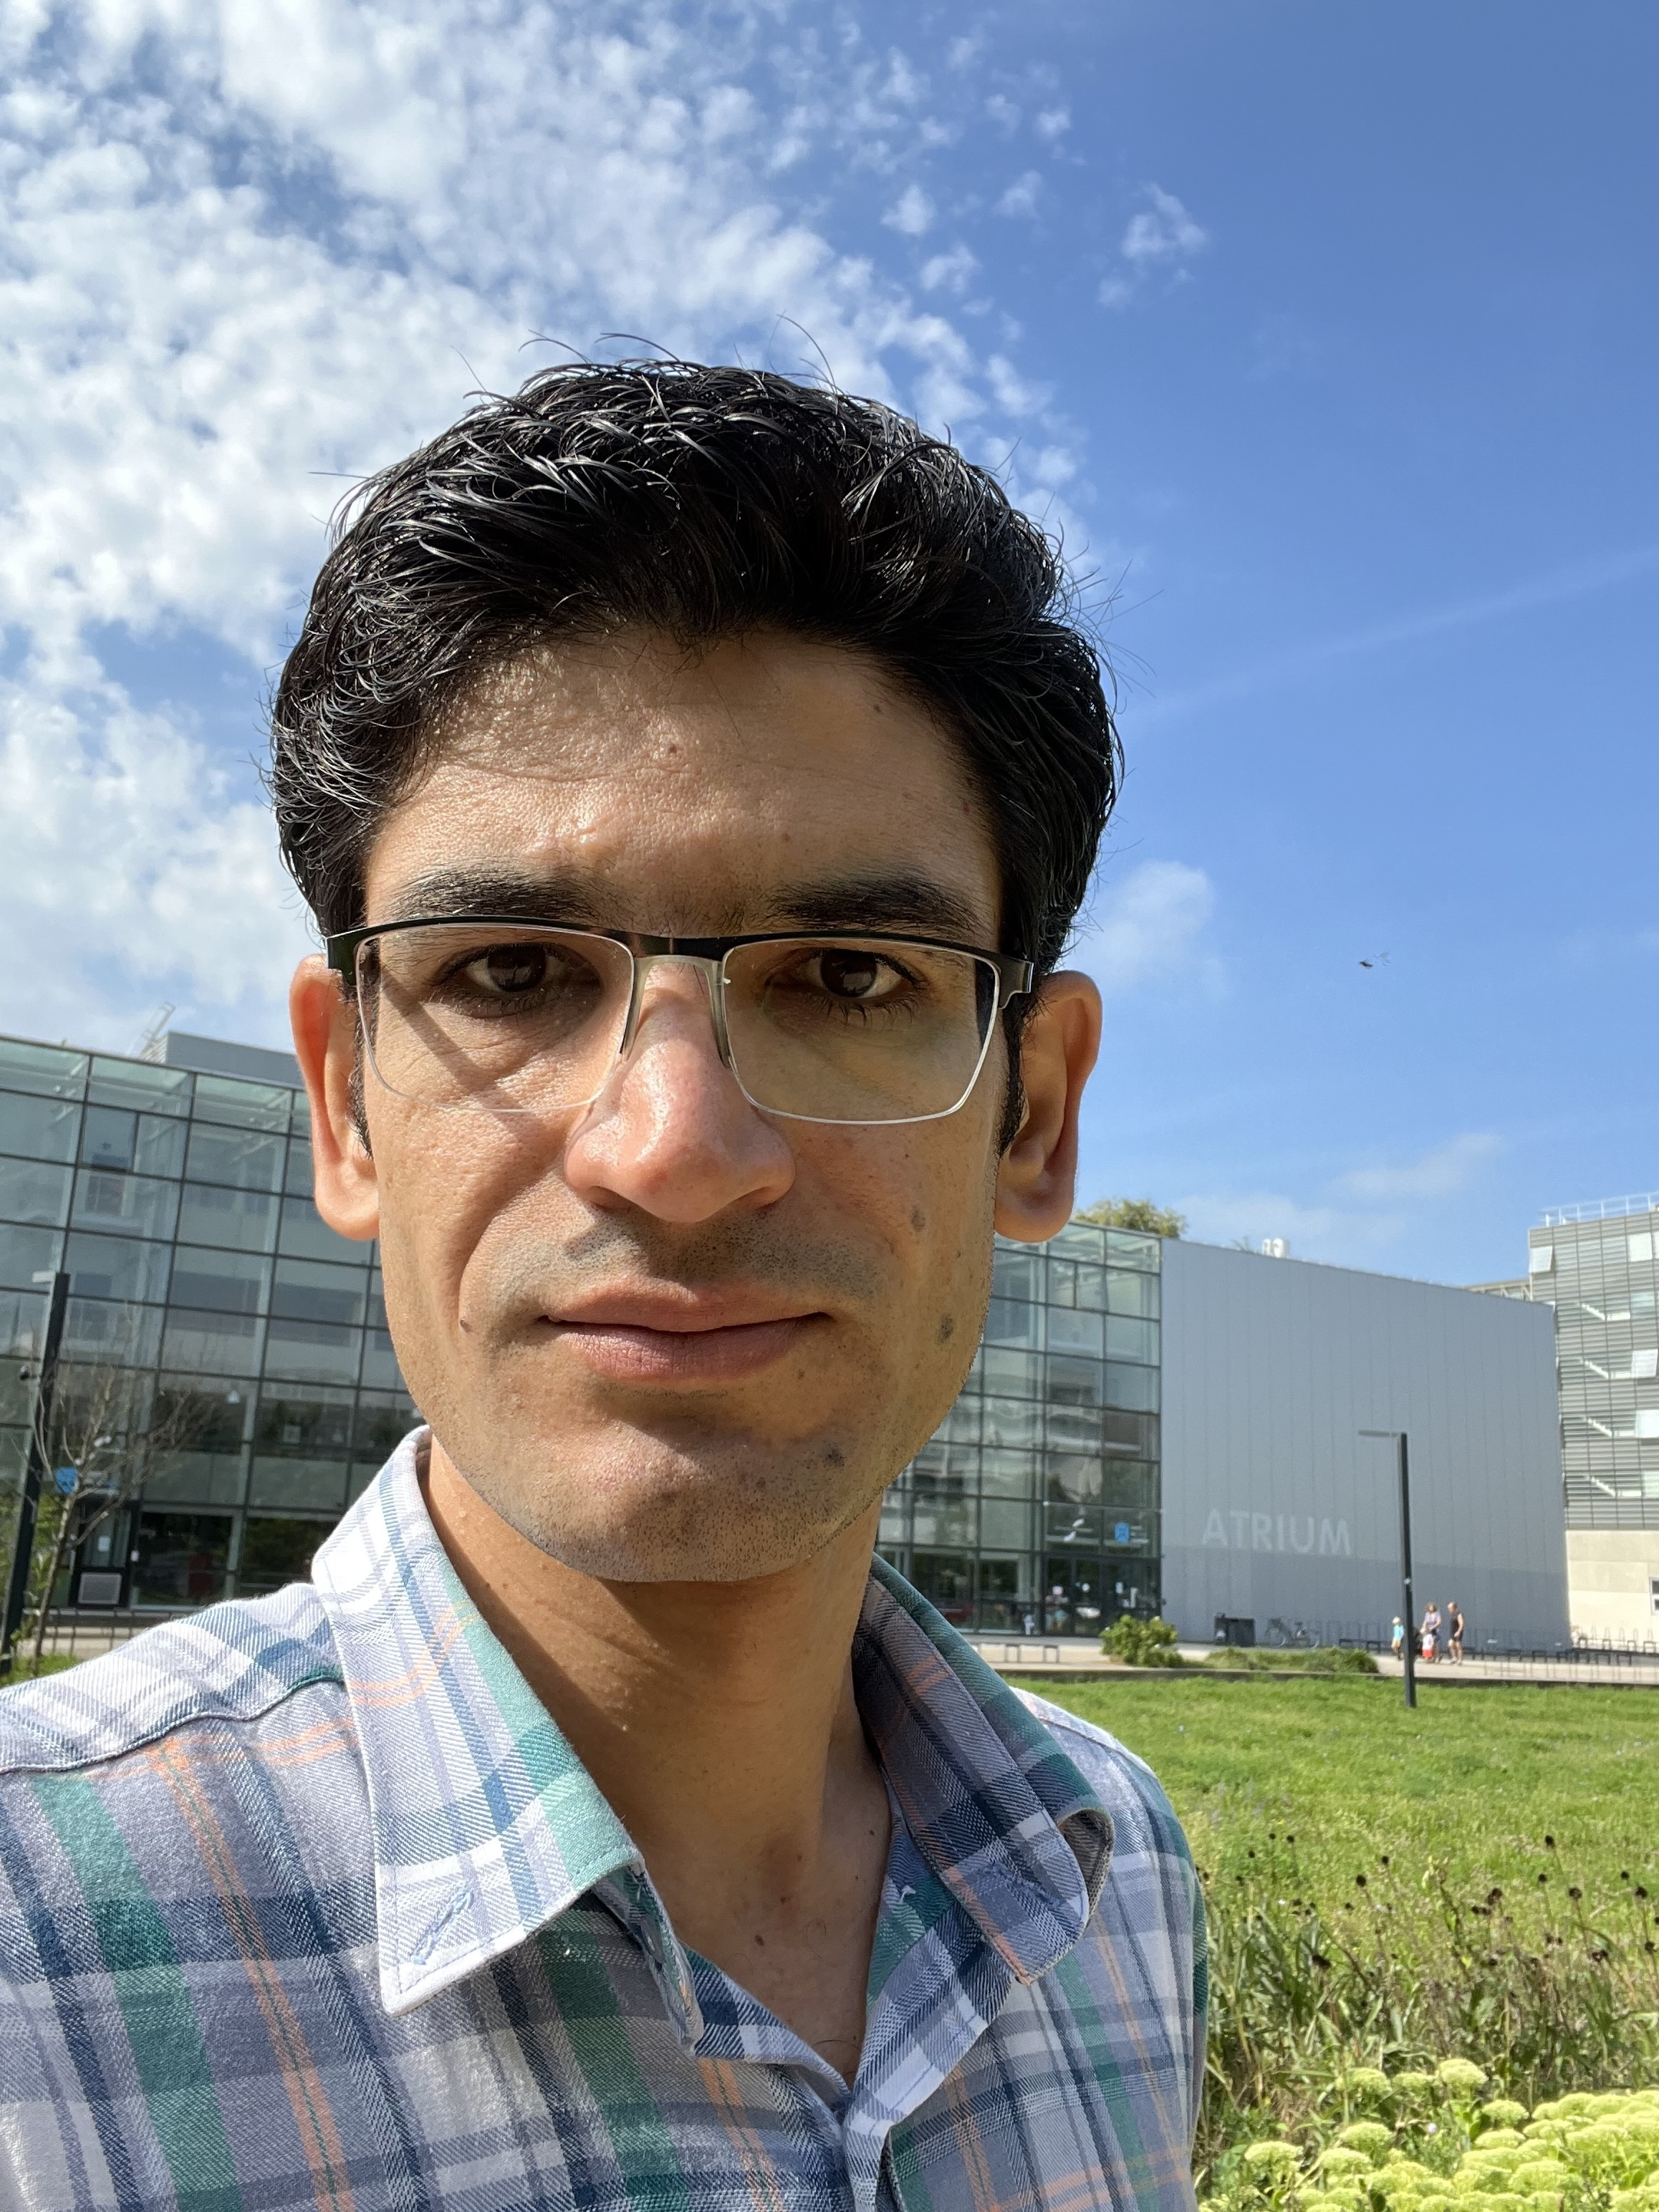
\includegraphics[width=4cm]{profile.jpg}};
\end{tikzpicture}

\vspace{5mm}

\divider

% ========================= Contact ===========================

\faPhone \quad 06 52 22 49 24

\faEnvelope \quad jafarizadeh89@gmail.com

\faGithub \quad \href{https://github.com/jafarizadeh}{jafarizadeh}

\faLinkedin \quad \href{https://www.linkedin.com/in/jafarizadeh/}{linkedin.com/in/jafarizadeh/}

\divider

% ================ Languages ================
{\large \textbf{Languages}}

\faCircleNotch \quad Persian (native)

\faCircleNotch \quad French (advanced level)

\faCircleNotch \quad English (intermediate level)

\divider

% ================ Programming Languages ================

{\large \textbf{Programming Languages}}

\faCircleNotch \quad Python

\faCircleNotch \quad C

\faCircleNotch \quad Swift

\faCircleNotch \quad HTML / CSS

\faCircleNotch \quad JavaScript

\faCircleNotch \quad SQL

\divider

% ===================== CAD Software ======================

{\large \textbf{CAD Software}}

\faCircleNotch \quad AutoCAD

\faCircleNotch \quad CATIA

\divider

% ========================== Network ==========================

{\large \textbf{Network}}

\faNetworkWired \quad CCNP-ENCOR (in progress)

\faNetworkWired \quad CCNP-ENARSI

\faNetworkWired \quad CCNA

\divider

% ===================== Driver's License ======================

{\large \textbf{Driver's License}}

\faCar \quad License B2

\divider

% ===================== Interests ======================

{\large \textbf{Interests}}

\faBicycle \quad Cycling

\faGamepad \quad Video games (Minecraft)

\end{minipage}
\hfill
\begin{minipage}[t]{0.60\textwidth}

% ============================================================
% ======================= Right  Side ========================
% ============================================================

\setlength{\baselineskip}{1.5\baselineskip}
\vspace{0.7cm}

{\huge Mehdi JAFARIZADEH}

\vspace{0.5cm}

% ========================= Education =========================

{\large \textbf{Education}}
\divider

{\textbf{Bachelor's Degree (3rd year) in Computer Science}}

{\footnotesize September 2021 - Present}

{\textit{University of Strasbourg, Strasbourg}}

 

\begin{itemize}
    \footnotesize
    \item Acquired skills: LAN/WAN network configuration and management, process management, Linux administration, complexity analysis, data structures.
\end{itemize}

\vspace{ 2mm}

{\textbf{Bachelor in Energy Engineering (equivalent to a Bachelor's degree)}}

{\footnotesize September 2014 - December 2018}

{\textit{Quchan University of Technology, Mashhad, Iran}}

 

\begin{itemize}
    \footnotesize
    \item Final project: Energy consumption in smart homes
    \item Acquired skills: Energy modeling, energy efficiency optimization, use of specialized software
\end{itemize}

\vspace{ 2mm}

{\textbf{Diploma in Accounting (2-year degree)}}

{\footnotesize September 2007 - December 2010}

{\textit{Azad University of Kerman, Kerman, Iran}}


\begin{itemize}
    \footnotesize
    \item Acquired skills: Financial analysis, regulatory compliance
\end{itemize}

\vspace{ 2mm}

% ================ Additional Training ==================

{\large \textbf{Additional Training}}
\divider
\vspace{4mm}
\begin{itemize}
    \footnotesize \item {\textbf{CCNP ENCOR 350-401:} Infrastructure architecture, security, and automation; (173 h)}
    \vspace{2mm}
    \footnotesize \item {\textbf{CCNP ENARSI 300-410:} Advanced EIGRP, OSPF, BGP routing and WAN networks;(134 h)}
    \vspace{2mm}
    \footnotesize \item {\textbf{CCNA 200-301:} Network fundamentals, configuration, and troubleshooting; (128 h)}
\end{itemize}
\vspace{ 2mm}

% ================ Professional Experience =================

{\large \textbf{Professional Experience}}
\divider

 
{\textbf{Internship: IT Department}}

{\footnotesize May 2010 - September 2010}
\begin{itemize}
    \footnotesize \item \textit{Aria-Etemad Accounting Firm}
   \newline
    Performed client accounting calculations using Microsoft Office (especially Excel). Developed advanced skills in Microsoft 365 and accounting calculations during this experience.
\end{itemize}

\vspace{ 2mm}
{\textbf{Internship: Research and Development Department}}

{\footnotesize June 2017 - September 2017}
\begin{itemize}
    \footnotesize \item \textit{Kerman and Kavian Cable Industry}
   \newline
    Conducted research on the thermal analysis and electrical conductivity of copper wires under the supervision of Dr. Abdollahi. Used tools such as ANSYS and SolidWorks to model and analyze technical data. Performed in-depth reviews of scientific articles to support research efforts.
\end{itemize}

\vspace{ 2mm}
{\textbf{Director of the Energy Engineering Association}}

{\footnotesize September 2015 - December 2017}
\begin{itemize}
   \footnotesize \item \textit{Quchan University of Technology, Mashhad}
   \newline
   Led educational workshops and organized scientific competitions within the Energy Engineering Association to promote renewable energies and raise awareness of energy efficiency issues.
\end{itemize}

\vspace{ 2mm}

{\textbf{Teaching Assistant}}

{\footnotesize September 2014 - December 2017}
\begin{itemize}
    \footnotesize \item \textit{Quchan University of Technology, Mashhad}
    \newline
    Served as a teaching assistant for Mathematics I, Mathematics II, and Energy Conversion: provided student support, explained key concepts, and assisted with coursework and exam preparation.
\end{itemize}

\vspace{ 2mm}

% ================ Academic Contributions ==================

{\large \textbf{Academic Contributions}}
\divider
\vspace{ 2mm}
\begin{itemize}
    \footnotesize \item {\textbf{Co-author}, \textit{Energy Audit Guide for Students of Quchan University, with Dr. Majid Mahdavian, published in 2019}}
\end{itemize}

\end{minipage}

% ========================== QR Code ==========================

\begin{tikzpicture}[remember picture,overlay]
    \node[anchor=south east,inner sep=0pt] at ($(current page.south west)+(6.5cm,+2.5cm)$) {
        
\includegraphics[width=2cm]{Documentation_FR.png}
    };
    
    \node[anchor=south east,inner sep=0pt] at ($(current page.south west)+(4cm,+2.5cm)$) {
        \begin{minipage}[t]{3.05cm} 
            \color{white} \scriptsize \href{https://drive.google.com/file/d/1jKjZWYadaikaPetkEmjoupWWh_w1sMKA/view?usp=drive_link}{Please click here or scan this QR code to access a detailed folder of my academic and professional contributions.}
        \end{minipage}
    };

    \node[anchor=south west,inner sep=0pt] at ($(current page.south west)+(0.8cm,1cm)$) {
        \begin{minipage}[t]{4cm}
            \tiny \textcolor{white}{Last updated: \today}
        \end{minipage}
    };
\end{tikzpicture}

\end{document}
